	En este capítulo presentamos el trabajo realizado de la aplicación web a través de la descripción de las distintas pantallas que la conforman, así como  su funcionamiento y los problemas que resuelve su implementación.

\section{Pantallas de la aplicación}
	A continuación describimos cada una de las pantallas, incluyendo las relaciones entre ellas.
%-----------------------------------------------------------------------
\subsection{Pantalla de inicio de sesión}
\subsubsection{Descripción}
%Descripción amplia de las funciones de la pantalla incluyendo la descripción de todos los botones y las validaciones con las que cuenta
	En esta pantalla el usuario puede autenticarse en la aplicación para acceder a su panel de correspondencia. Contiene un campo de texto para introducir su correo con el cual se autenticará, otro campo de texto para introducir la contraseña y un botón de "Iniciar sesión" para que la aplicación haga la validación de los datos introducidos y de acceso al usuario. La figura \ref{fig:Autenticacion} muestra el diseño de esta pantalla.		
		
	\begin{figure}[htbp!]
		\centering
			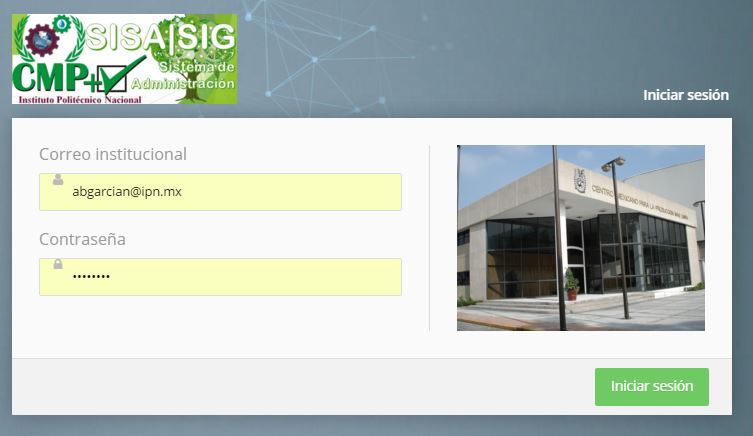
\includegraphics[width=0.8\textwidth]{Pantallas/iniciodesesion}
		\caption{Pantalla de inicio de sesión.}
		\label{fig:Autenticacion}
	\end{figure}

\subsubsection{Funcionamiento}
	Esta pantalla funciona de la siguiente manera:
	
	\begin{enumerate}
		\item El usuario ingresa su correo institucional y su contraseña.
		\item El usuario da clic en ``Aceptar''.
		\item La aplicación valida los datos introducidos.
		\item Si los datos son válidos entonces redirige al usuario a la pantalla de la figura \ref{fig:HomePage}.
		\item \item Si los datos no son válidos la aplicación redirije a la misma pantalla de la figura \ref{fig:Autenticacion}, con el mensage de ``Usuario o contraseña incorrectos. Verifique su correo y/o contraseña.''.
	\end{enumerate}

\subsubsection{Problemas que resuelve}
Esta pantalla ayuda a mitigar las causas que dan origen a los siguientes problemas:

	\begin{itemize}
		\item Saber quién está atendiendo los diferentes oficios y memorándums del CMPL.
		\item Saber quién tiene en determinado momento un oficio o un memorándum.
	\end{itemize}

\subsubsection{Pantallas relacionadas}
Está pantalla se relaciona con las siguientes figuras de pantallas:
	\begin{itemize}
		\item \ref{fig:HomePage}
	\end{itemize}
%-----------------------------------------------------------------------
\subsection{Pantalla de página principal}
\subsubsection{Descripción}
%Descripción amplia de las funciones de la pantalla incluyendo la descripción de todos los botones y las validaciones con las que cuenta
	En esta pantalla el usuario puede ver un concentrado de toda su correspondencia, es decir, todos los oficios y memorándums, ordenados del más actual al más antiguo, viendo el tipo de correspondencia que es (oficio o memorándum), la fecha en la cual le fue turnado, el emisor de dicha correspondencia, el asunto y el menú de acciones. La figura \ref{fig:HomePage} muestra el diseño de esta pantalla.		
		
	\begin{figure}[htbp!]
		\centering
			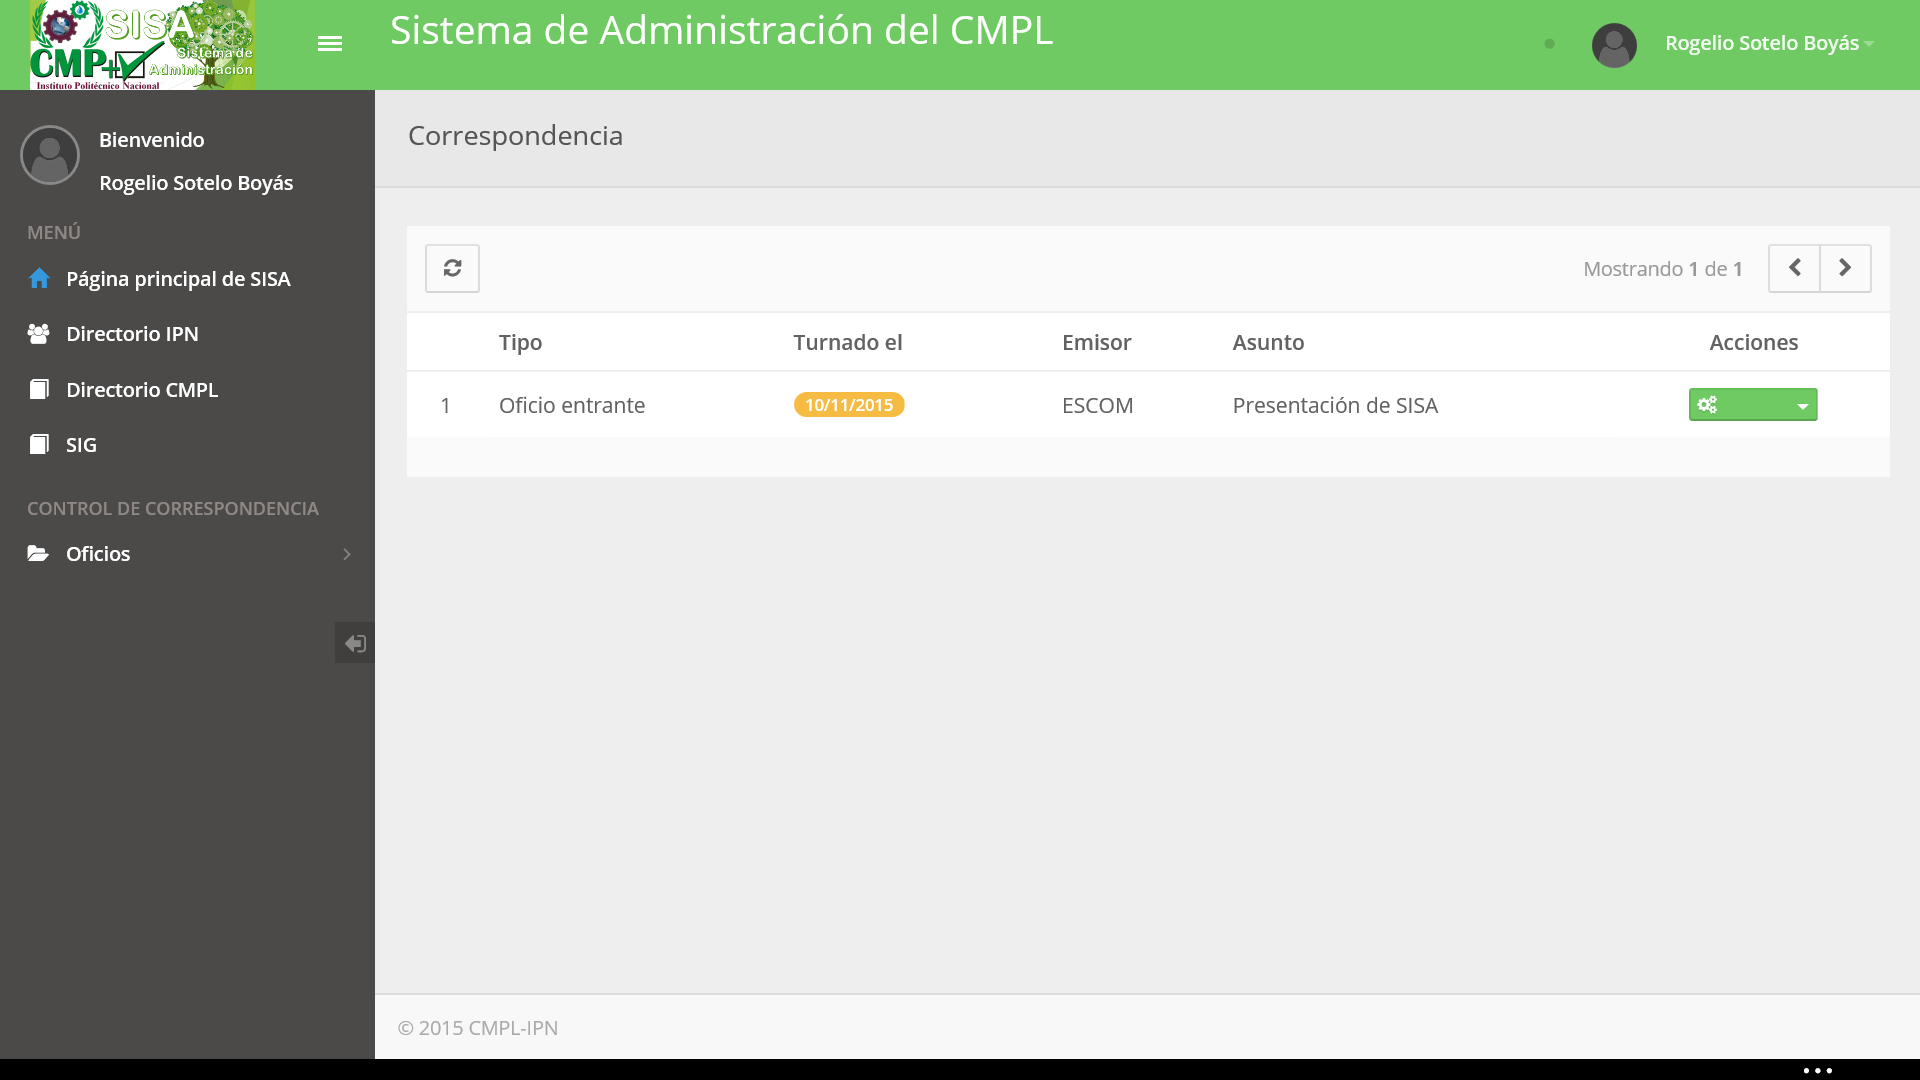
\includegraphics[width=1\textwidth]{Pantallas/PaginaPrincipal.png}
		\caption{Pantalla de página principal.}
		\label{fig:HomePage}
	\end{figure}

\subsubsection{Funcionamiento}
	Esta pantalla funciona de la siguiente manera:
	
	\begin{enumerate}
		\item El usuario da clic sobre la correspondencia que desea revisar.
		\item La aplicación muestra la copia en PDF del oficio o memorándum seleccionado.
	\end{enumerate}

\subsubsection{Problemas que resuelve}
Esta pantalla ayuda a mitigar las causas que dan origen a los siguientes problemas:

	\begin{itemize}
		\item No se sabe cuándo llegó correspondencia y qué día fue turnado.
		\item No siempre se informa al destinatario la llegada de correspondencia.
		\item El registro de los oficios y memorándums no se realiza de forma correcta.
	\end{itemize}

\subsubsection{Pantallas relacionadas}
Está pantalla se relaciona con las siguientes figuras de pantallas:
	\begin{itemize}
		\item \ref{fig:OficiosEntrantes}
	\end{itemize}

%-----------------------------------------------------------------------
\subsection{Pantalla de oficios entrantes}
\subsubsection{Descripción}
%Descripción amplia de las funciones de la pantalla incluyendo la descripción de todos los botones y las validaciones con las que cuenta
	En esta pantalla se muestra el concentrado de todos los oficios entrantes que se han registrado, mostrando su número de oficio, la dependencia que lo emitió, el asunto, la fecha de entrega y las acciones del oficio. La figura \ref{fig:OficiosEntrantes} muestra el diseño de esta pantalla.		
		
	\begin{figure}[htbp!]
		\centering
			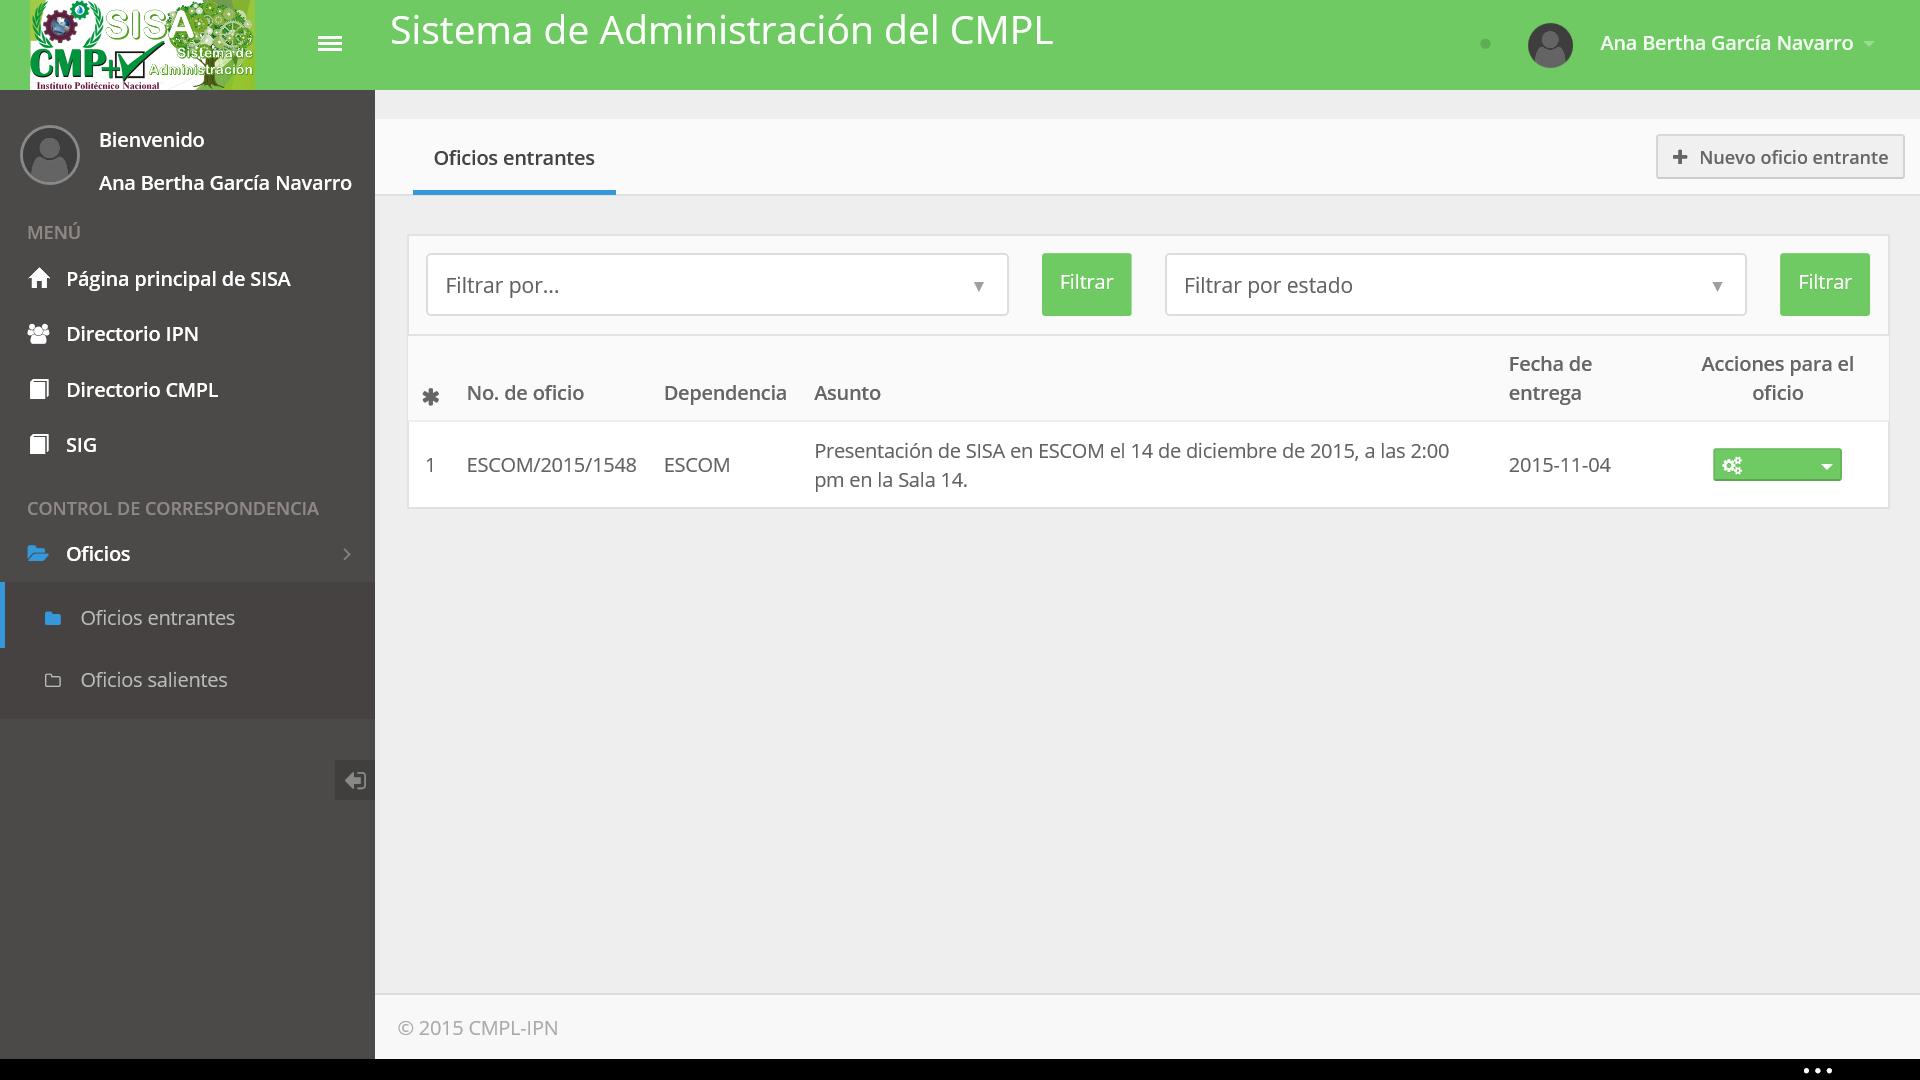
\includegraphics[width=1\textwidth]{Pantallas/OficiosEntrantes.png}
		\caption{Pantalla de oficios entrantes.}
		\label{fig:OficiosEntrantes}
	\end{figure}

\subsubsection{Funcionamiento}
	Esta pantalla funciona de la siguiente manera:
	
	\begin{enumerate}
		\item El usuario puede seleccionar el tipo de filtro que mejor le convenga, y sea por consecutivo, por fecha de recepción, por dependencia o por estado.
		\item El usuario le da clic en ``Filtrar''.
		\item La aplicación aplica el filtro.
		\item La aplicación muestra los oficios entrantes con el filtro correspondiente.
	\end{enumerate}

\subsubsection{Problemas que resuelve}
Esta pantalla ayuda a mitigar las causas que dan origen a los siguientes problemas:

	\begin{itemize}
		\item No se sabe cuál es el estatus de los oficios.
		\item El registro de los oficios no se lleva de forma correcta.
		\item Es complicado saber el orden de llegada de los oficios entrantes.
	\end{itemize}

\subsubsection{Pantallas relacionadas}
Está pantalla se relaciona con las siguientes figuras de pantallas:
	\begin{itemize}
		\item \ref{fig:Wizard1DatosDelRemitente}
	\end{itemize}

%-----------------------------------------------------------------------
\subsection{Pantalla de datos del remitente de oficios entrantes}
\subsubsection{Descripción}
%Descripción amplia de las funciones de la pantalla incluyendo la descripción de todos los botones y las validaciones con las que cuenta
	En esta pantalla, que es la pantalla inicial de un registro de oficio entrante, muestra una sección especial donde se puede administrar el registro de los datos del remitente como su cargo, área y la dependencia que está mandando el oficio . La figura \ref{fig:Wizard1DatosDelRemitente} muestra el diseño de esta pantalla.		
		
	\begin{figure}[htbp!]
		\centering
			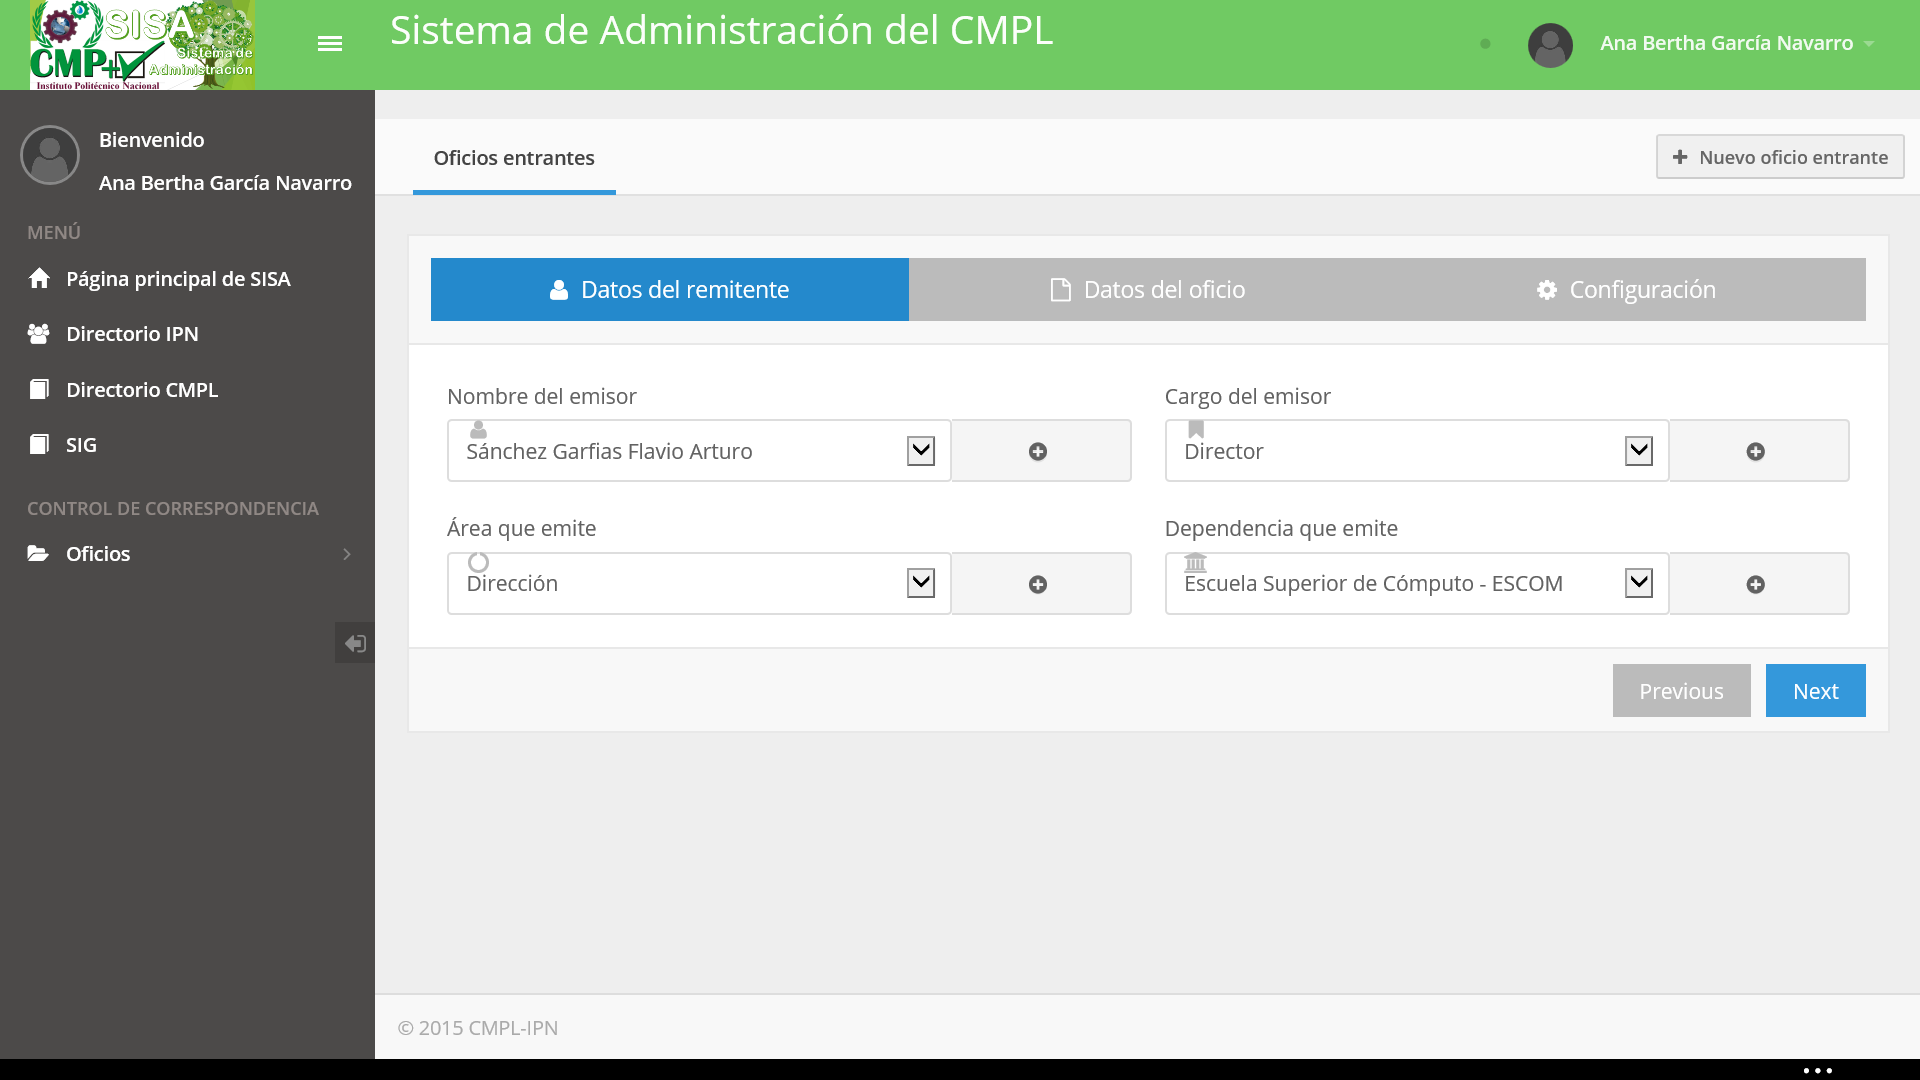
\includegraphics[width=1\textwidth]{Pantallas/Wizard1DatosDelRemitente.png}
		\caption{Pantalla de datos del remitente de oficios entrantes.}
		\label{fig:Wizard1DatosDelRemitente}
	\end{figure}

\subsubsection{Funcionamiento}
	Esta pantalla funciona de la siguiente manera:
	
	\begin{enumerate}
		\item La aplicación muestra catálogos para elegir el remitente, su cargo, su área y su dependencia.
		\item El usuario selecciona de los catálogos la información requerida.
		\item Si el usuario no llegara a encontrar la información deseada, puede darla de alta haciendo clic en ``+'' del tipo de información nueva que desea registrar.
		\item El usuario da clic en ``Next''.
	\end{enumerate}

\subsubsection{Problemas que resuelve}
Esta pantalla ayuda a mitigar las causas que dan origen a los siguientes problemas:

	\begin{itemize}
		\item Es complicado saber de forma inmediata quién está emitiendo un oficio entrante.
		\item Es complicado organizar los oficios entrantes por dependencias, áreas o departamentos de las entidades que emiten.
	\end{itemize}

\subsubsection{Pantallas relacionadas}
Está pantalla se relaciona con las siguientes figuras de pantallas:
	\begin{itemize}
		\item \ref{fig:Wizard2DatosDelOficio}
		\item \ref{fig:NuevoEmisor}
		\item \ref{fig:NuevoCargoEmisor}
		\item \ref{fig:NuevaAreaEmisor}
		\item \ref{fig:NuevaDependencia}
	\end{itemize}

%-----------------------------------------------------------------------
\subsection{Pantalla de datos del oficio de oficios entrantes}
\subsubsection{Descripción}
%Descripción amplia de las funciones de la pantalla incluyendo la descripción de todos los botones y las validaciones con las que cuenta
	En esta pantalla el usuario puede ingresar el número de oficio, a quién va dirigido, la fecha de emisión y recepción del oficio y el asunto. La figura \ref{fig:Wizard2DatosDelOficio} muestra el diseño de esta pantalla.		
		
	\begin{figure}[htbp!]
		\centering
			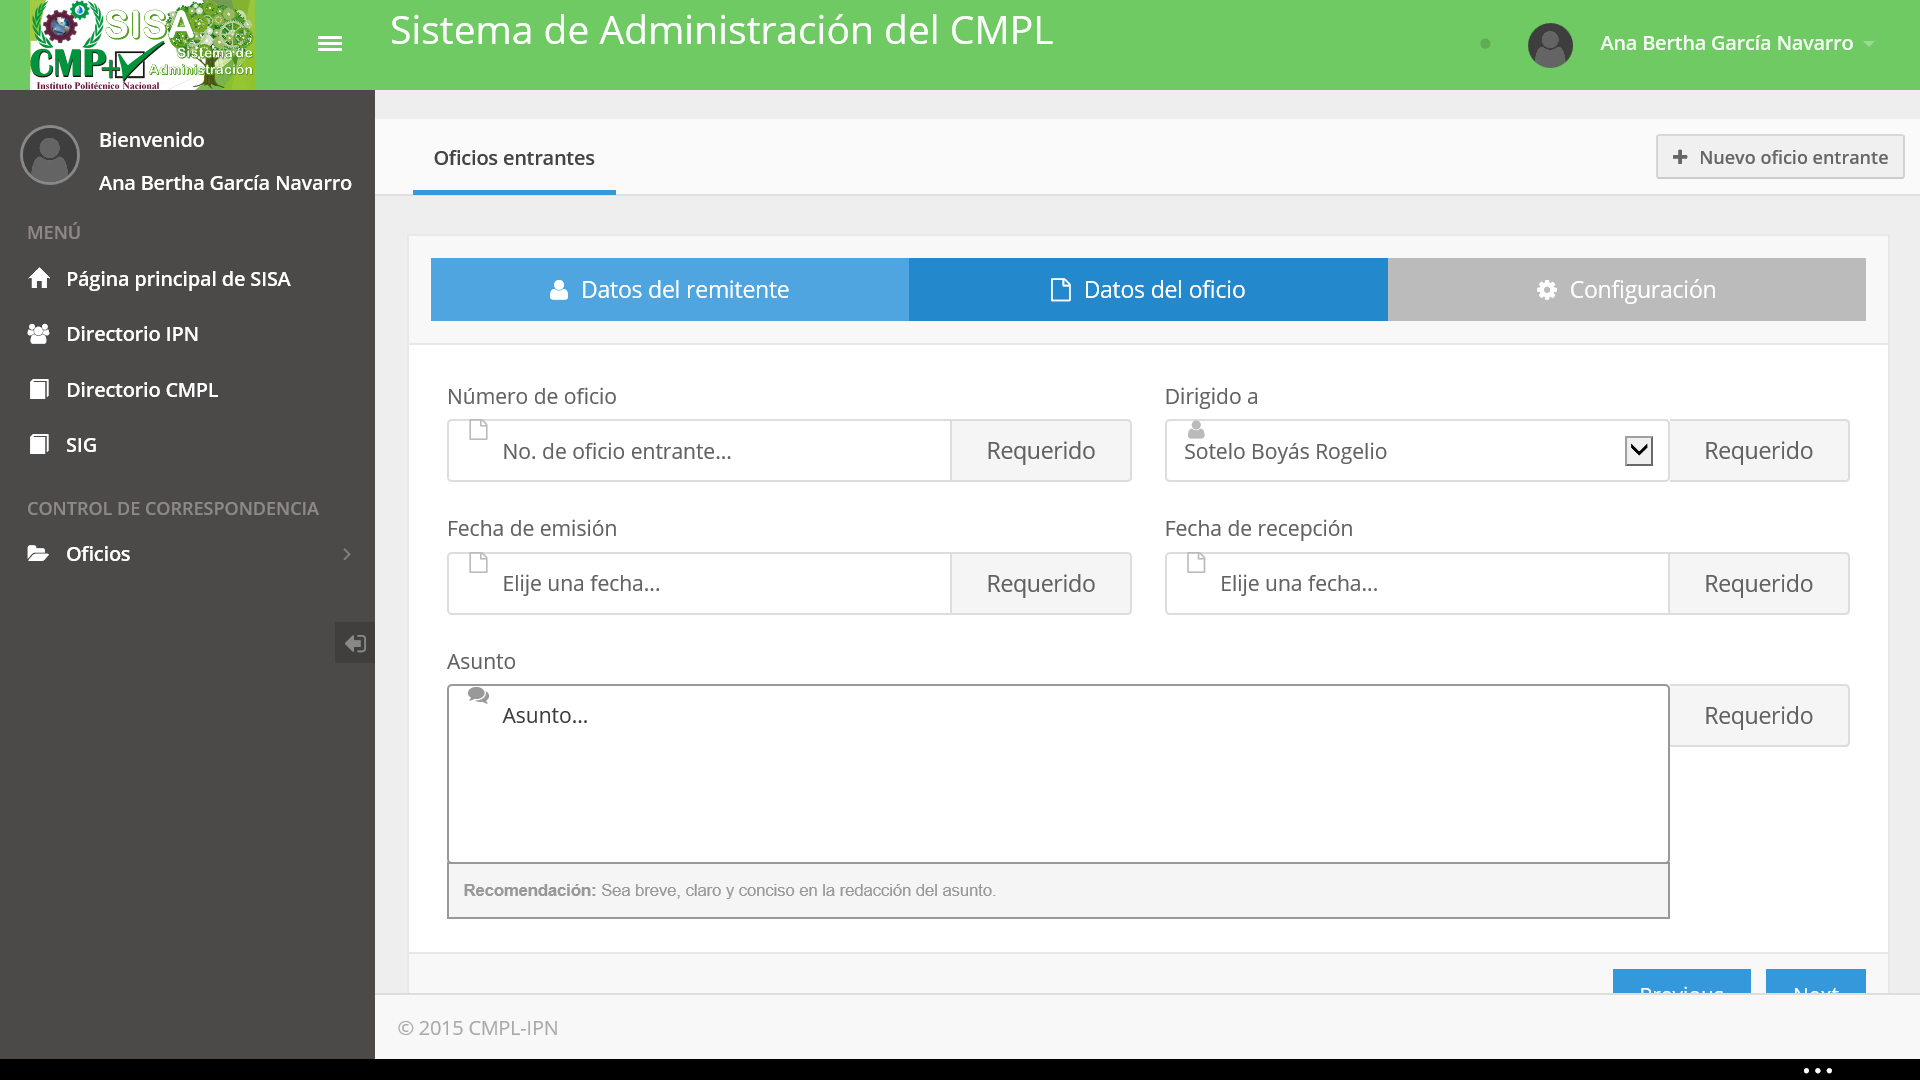
\includegraphics[width=1\textwidth]{Pantallas/Wizard2DatosDelOficio.png}
		\caption{Pantalla de datos del emisor de oficios entrantes.}
		\label{fig:Wizard2DatosDelOficio}
	\end{figure}

\subsubsection{Funcionamiento}
	Esta pantalla funciona de la siguiente manera:
	
	\begin{enumerate}
		\item El usuario ingresa los datos soliticados por la aplicación en esta pantalla.
		\item El usuario da clic en ``Next''.
	\end{enumerate}

\subsubsection{Problemas que resuelve}
Esta pantalla ayuda a mitigar las causas que dan origen a los siguientes problemas:

	\begin{itemize}
		\item El registro de oficios no se realiza de forma correcta.
	\end{itemize}

\subsubsection{Pantallas relacionadas}
Está pantalla se relaciona con las siguientes figuras de pantallas:
	\begin{itemize}
		\item \ref{fig:Wizard1DatosDelRemitente}
		\item \ref{fig:Wizard3Configuracion}
	\end{itemize}

%-----------------------------------------------------------------------
\subsection{Pantalla de configuración de oficios entrantes}
\subsubsection{Descripción}
%Descripción amplia de las funciones de la pantalla incluyendo la descripción de todos los botones y las validaciones con las que cuenta
	En esta pantalla el usuario puede configurar el oficio, es decir, si es un oficio de respuesta a un oficio saliente registrado anteriormente, si éste requiere respuesta, así como subir el documento en PDF del oficio físico. La figura \ref{fig:Wizard3Configuracion} muestra el diseño de esta pantalla.		
		
	\begin{figure}[htbp!]
		\centering
			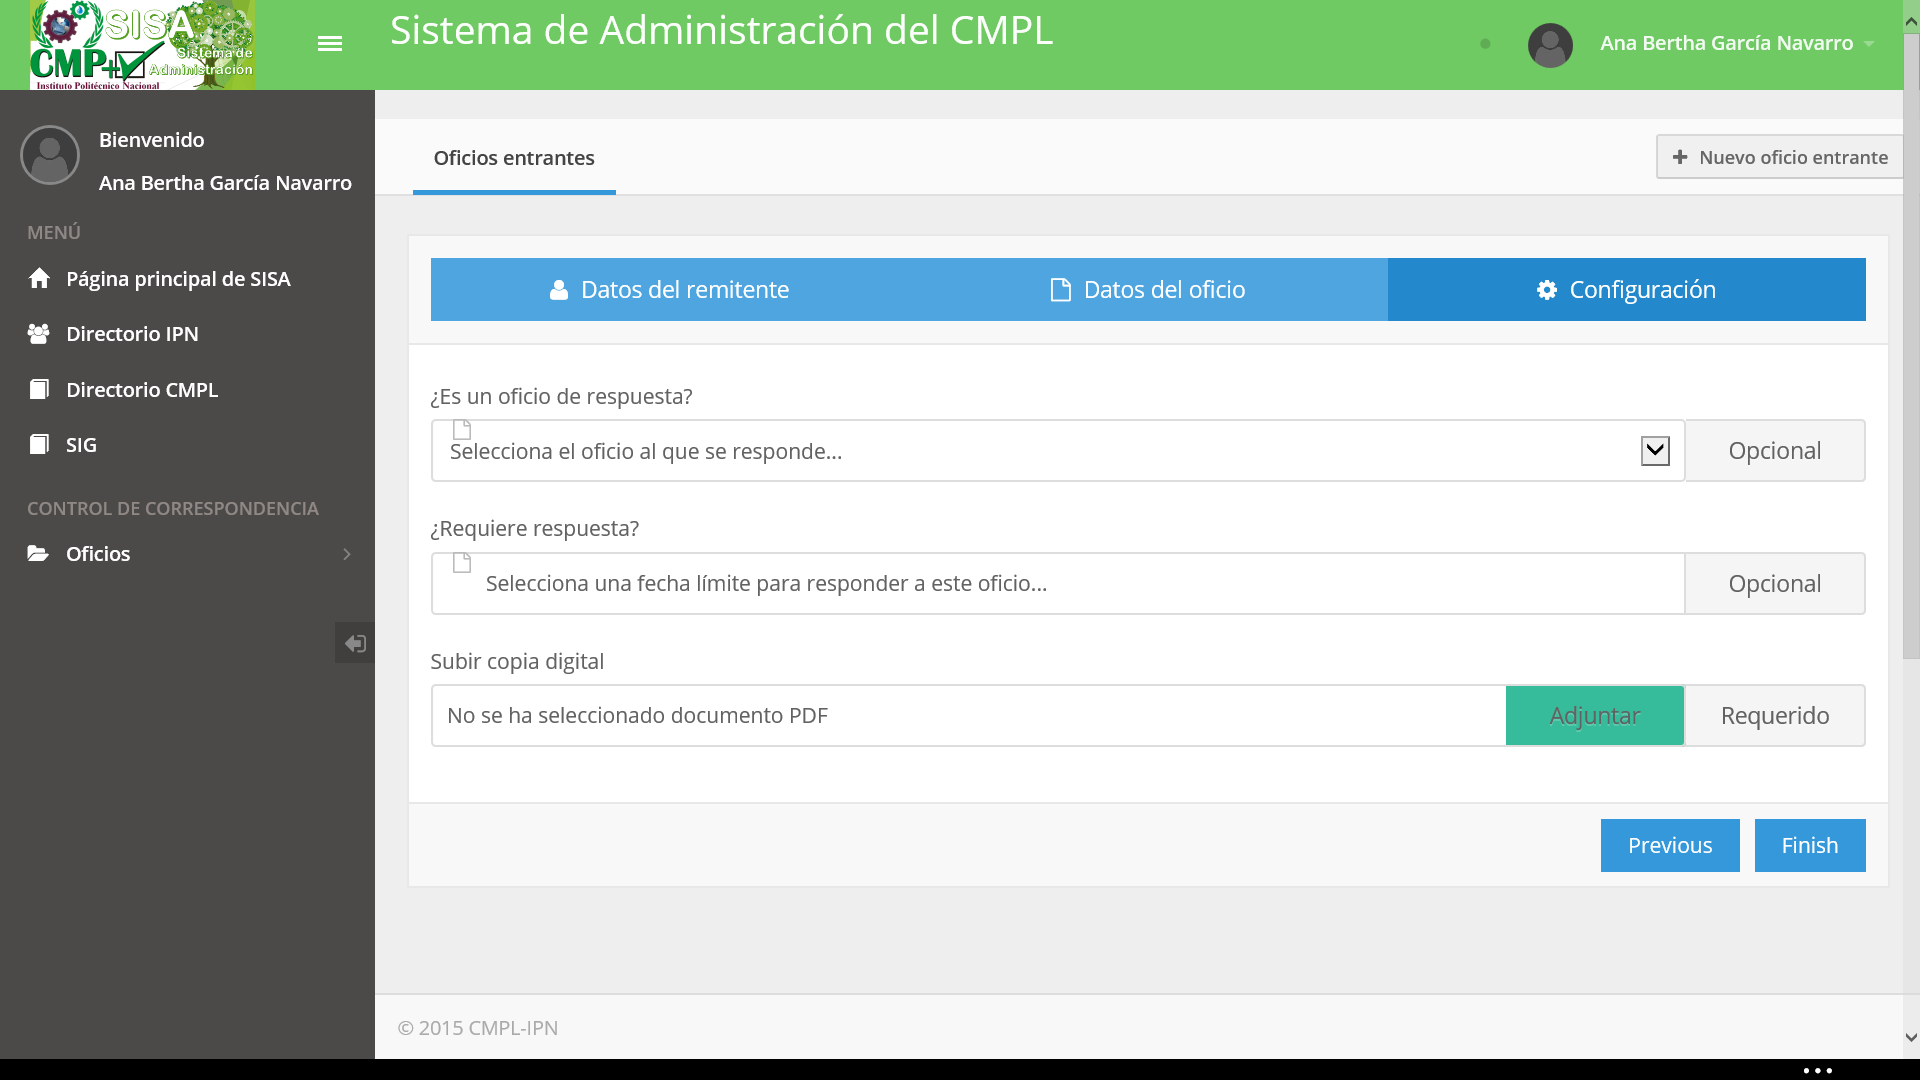
\includegraphics[width=1\textwidth]{Pantallas/Wizard3Configuracion.png}
		\caption{Pantalla de configuración de oficios entrantes.}
		\label{fig:Wizard3Configuracion}
	\end{figure}

\subsubsection{Funcionamiento}
	Esta pantalla funciona de la siguiente manera:
	
	\begin{enumerate}
		\item El usuario elije si es o no un oficio de respuesta a un oficio saliente registrado anteriormente.
		\item Si tiene fecha límite de respuesta entonces el usuario registra dicha fecha.
		\item Selecciona de su computadora el archivo en formato PDF para subirlo a la aplicación.
		\item El usuario da clic en ``Finish''.
		\item La aplicación valida los datos ingresados.
		\item Si son válidos los datos ingresados, la aplicación registra el oficio entrante.
		\item Si no son válidos los datos ingresados entonces la aplicación muestra la pantalla de la figura \ref{fig:Wizard1DatosDelRemitente}, con los errores de validación encontrados.
	\end{enumerate}

\subsubsection{Problemas que resuelve}
Esta pantalla ayuda a mitigar las causas que dan origen a los siguientes problemas:

	\begin{itemize}
		\item Es complicado saber la ubicación física del oficio entrante.
		\item No se tiene un registro de la fecha límite de respuesta al instante.
		\item Es complicado determinar si el oficio originalmente tenía fecha límite de respuesta.
		\item Se puede perder la certificación de la ISO 14000 al no contar con un sistema que les permita reducir consumo de papel en el manejo de oficios del CMPL.
	\end{itemize}

\subsubsection{Pantallas relacionadas}
Está pantalla se relaciona con las siguientes figuras de pantallas:
	\begin{itemize}
		\item \ref{fig:Wizard1DatosDelRemitente}
		\item \ref{fig:Wizard2DatosDelOficio}
	\end{itemize}

%-----------------------------------------------------------------------
\subsection{Pantalla de registro de emisor de oficios entrantes}
\subsubsection{Descripción}
%Descripción amplia de las funciones de la pantalla incluyendo la descripción de todos los botones y las validaciones con las que cuenta
	En esta pantalla el usuario puede registrar el nombre y cargo del remitente que envió el oficio en caso de que aún no exista su registro dentro de la aplicación. La figura \ref{fig:NuevoEmisor} muestra el diseño de esta pantalla.		
		
	\begin{figure}[htbp!]
		\centering
			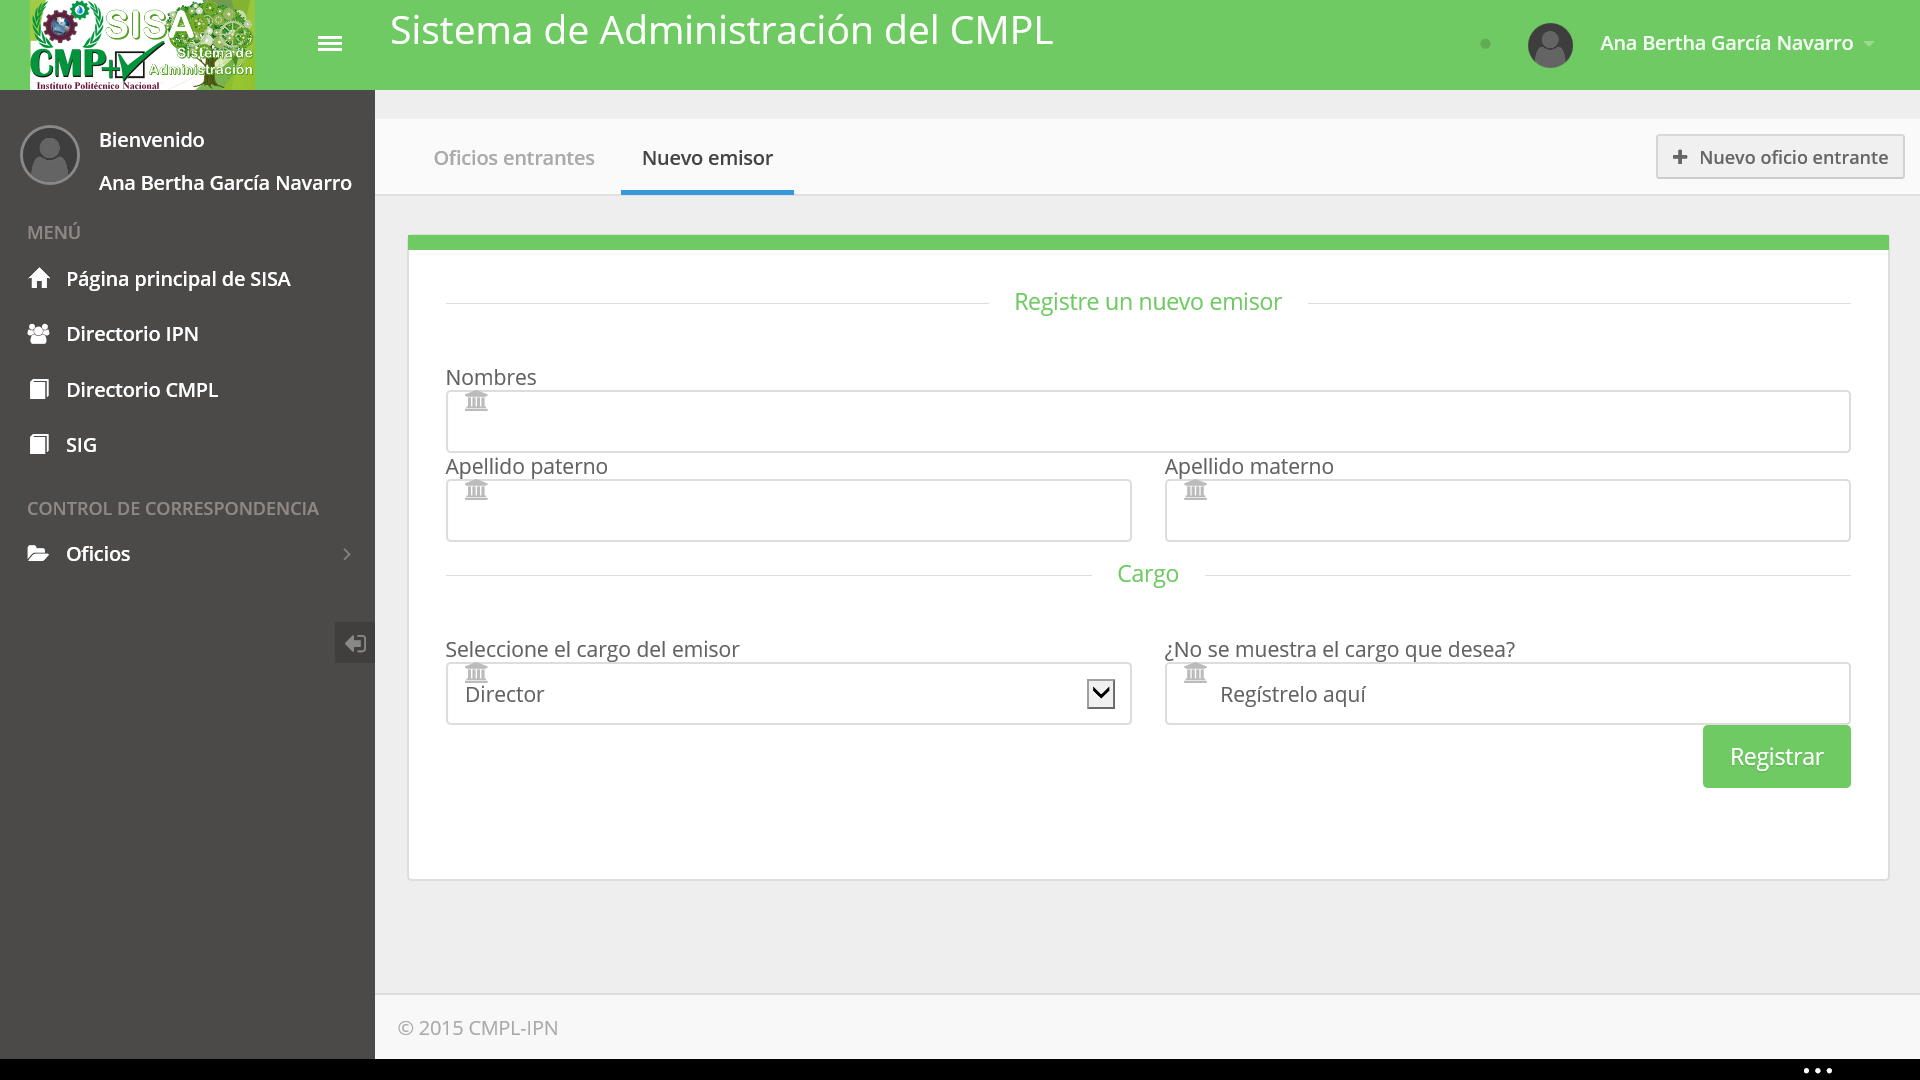
\includegraphics[width=1\textwidth]{Pantallas/NuevoEmisor.png}
		\caption{Pantalla de registro de emisor de oficios entrantes.}
		\label{fig:NuevoEmisor}
	\end{figure}

\subsubsection{Funcionamiento}
	Esta pantalla funciona de la siguiente manera:
	
	\begin{enumerate}
		\item El usuario ingresa el o los nombres del emisor, sus apellidos y su cargo, ya sea seleccionándolo del menú de cargos, o bien, registrando un nuevo cargo.
		\item El usuario da clic en ``Registrar''.
		\item La aplicación valida que todos los campos requeridos estén llenos.
		\item La aplicación registra la información ingresada.
		\item La aplicación vuelve a la pantalla de la figura \ref{fig:Wizard1DatosDelRemitente}, con el registro del nuevo remitente.
	\end{enumerate}

\subsubsection{Problemas que resuelve}
Esta pantalla ayuda a mitigar las causas que dan origen a los siguientes problemas:

	\begin{itemize}
		\item Es complicado consultar todos los oficios que un remitente ha enviado al CMPL.
	\end{itemize}

\subsubsection{Pantallas relacionadas}
Está pantalla se relaciona con las siguientes figuras de pantallas:
	\begin{itemize}
		\item \ref{fig:Wizard1DatosDelRemitente}
	\end{itemize}

%-----------------------------------------------------------------------
\subsection{Pantalla de registro de cargo del emisor de oficios entrantes}
\subsubsection{Descripción}
%Descripción amplia de las funciones de la pantalla incluyendo la descripción de todos los botones y las validaciones con las que cuenta
	En esta pantalla el usuario puede registrar el nombre del cargo del remitente que envió el oficio en caso de que aún no exista su registro dentro de la aplicación. La figura \ref{fig:NuevoCargoEmisor} muestra el diseño de esta pantalla.		
		
	\begin{figure}[htbp!]
		\centering
			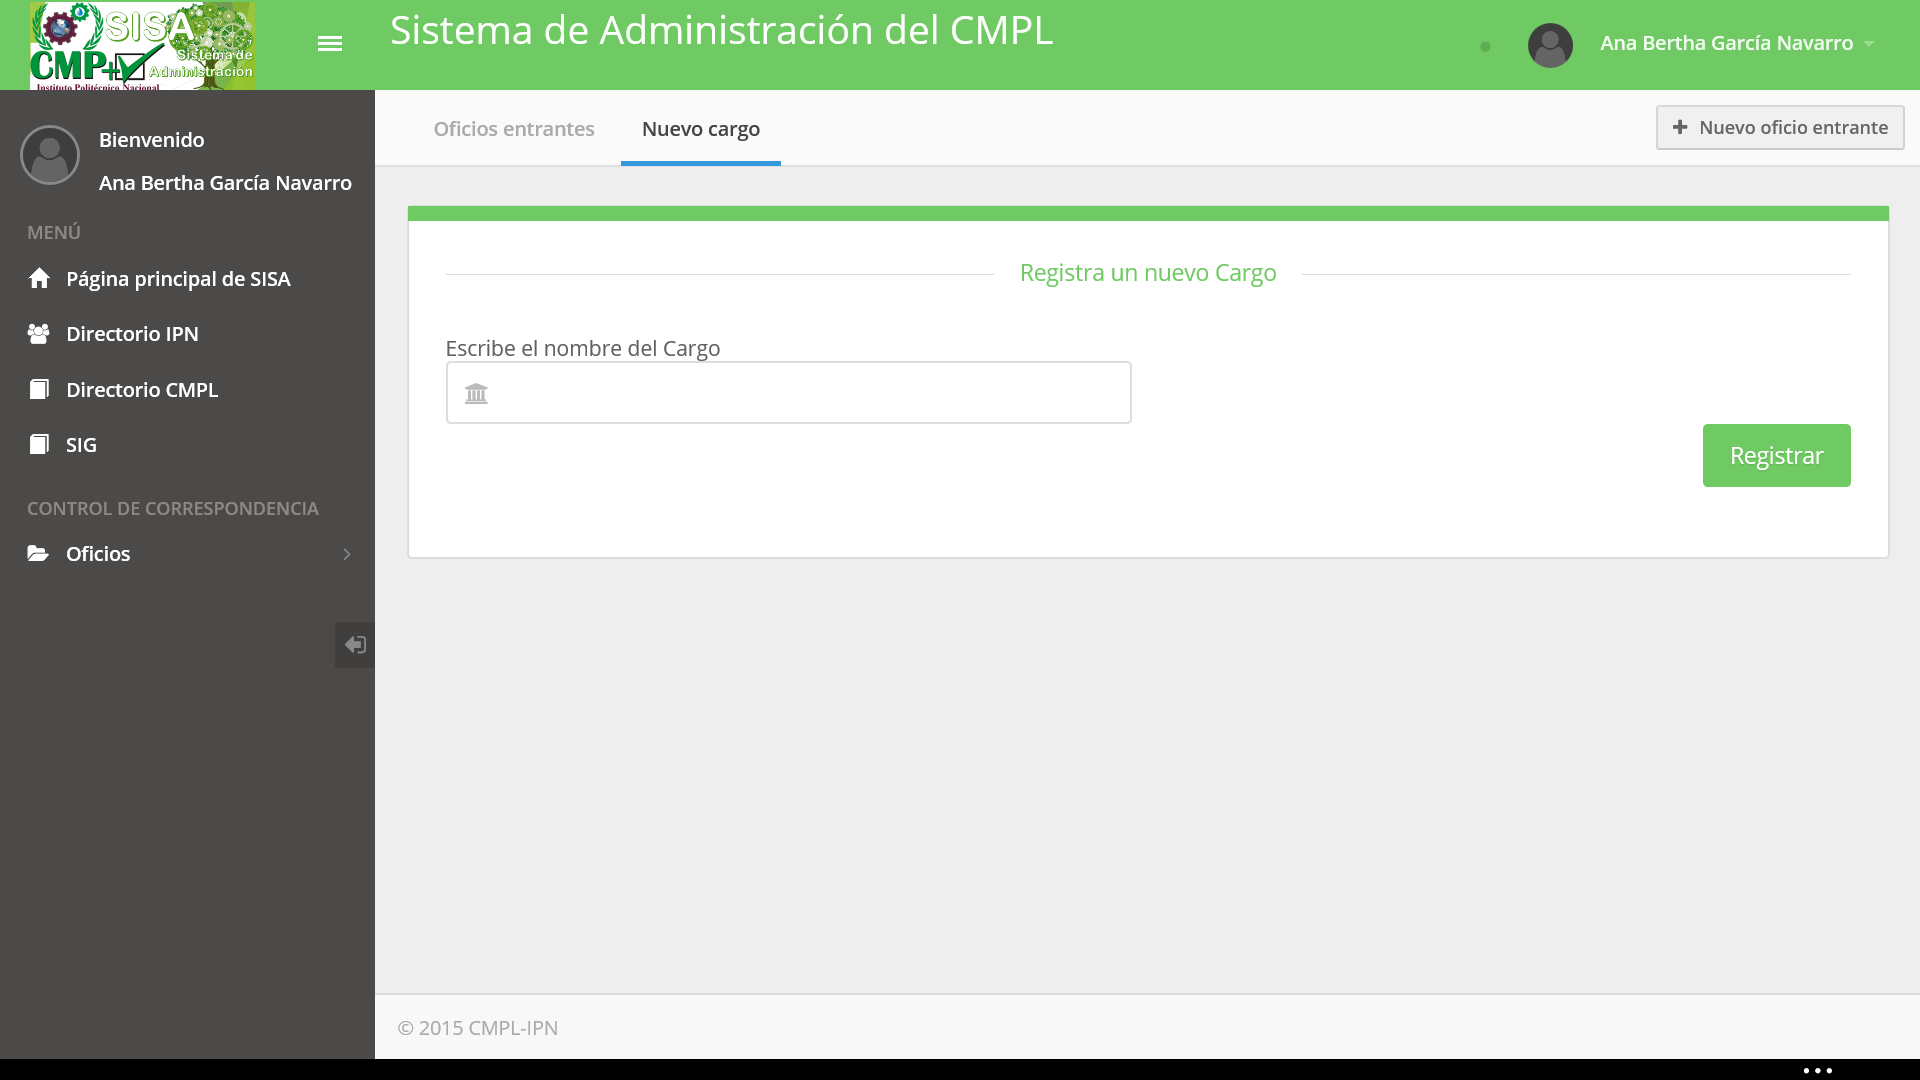
\includegraphics[width=1\textwidth]{Pantallas/NuevoCargoEmisor.png}
		\caption{Pantalla de registro de cargo del emisor de oficios entrantes.}
		\label{fig:NuevoCargoEmisor}
	\end{figure}

\subsubsection{Funcionamiento}
	Esta pantalla funciona de la siguiente manera:
	
	\begin{enumerate}
		\item El usuario ingresa el nombre del cargo del emisor.
		\item El usuario da clic en ``Registrar''.
		\item La aplicación valida que todos los campos requeridos estén llenos.
		\item La aplicación registra la información ingresada.
		\item La aplicación vuelve a la pantalla de la figura \ref{fig:Wizard1DatosDelRemitente}, con el registro del nuevo cargo del remitente.
	\end{enumerate}

\subsubsection{Problemas que resuelve}
Esta pantalla ayuda a mitigar las causas que dan origen a los siguientes problemas:

	\begin{itemize}
		\item Es complicado consultar todos los oficios que un remitente con cierto cargo ha enviado al CMPL.
	\end{itemize}

\subsubsection{Pantallas relacionadas}
Está pantalla se relaciona con las siguientes figuras de pantallas:
	\begin{itemize}
		\item \ref{fig:Wizard1DatosDelRemitente}
	\end{itemize}

%-----------------------------------------------------------------------
\subsection{Pantalla de registro de área que emite de oficios entrantes}
\subsubsection{Descripción}
%Descripción amplia de las funciones de la pantalla incluyendo la descripción de todos los botones y las validaciones con las que cuenta
	En esta pantalla el usuario puede registrar el nombre del área del remitente que envió el oficio en caso de que aún no exista su registro dentro de la aplicación. La figura \ref{fig:NuevaAreaEmisor} muestra el diseño de esta pantalla.		
		
	\begin{figure}[htbp!]
		\centering
			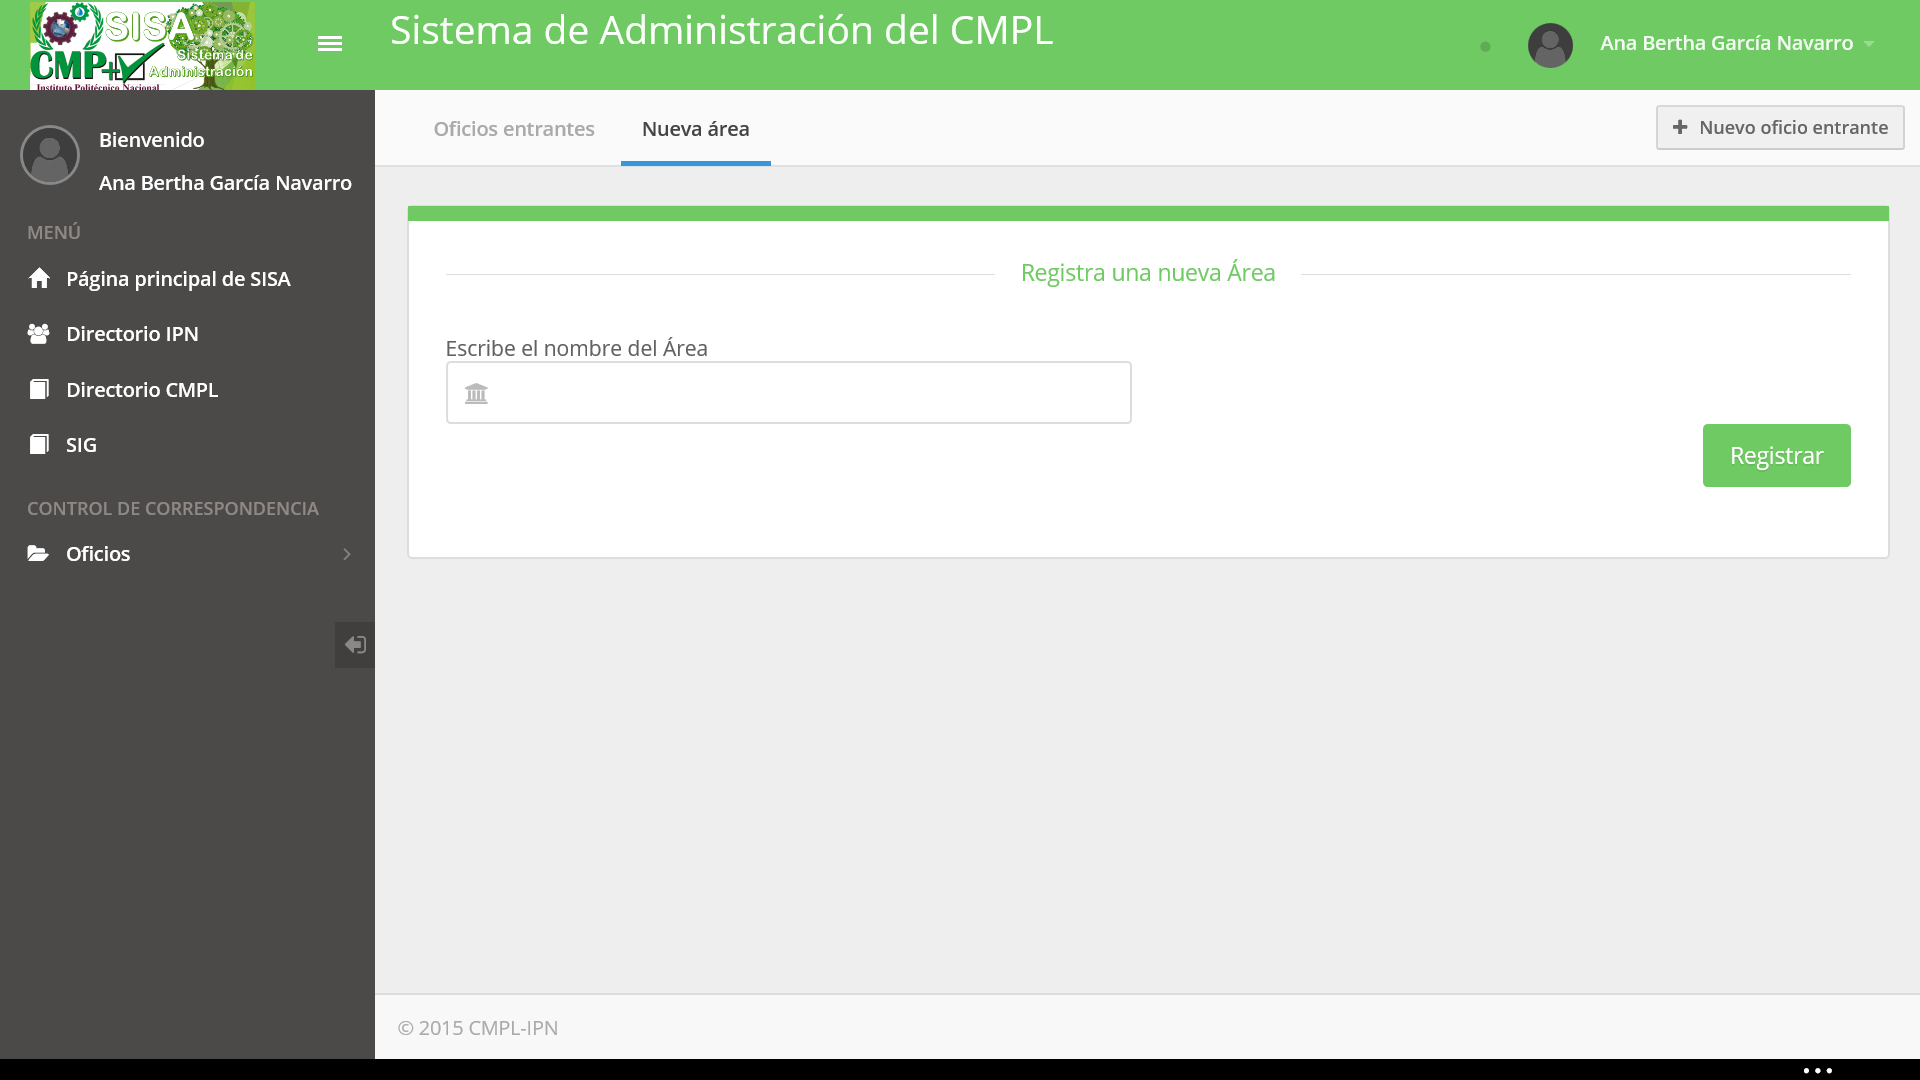
\includegraphics[width=1\textwidth]{Pantallas/NuevaAreaEmisor.png}
		\caption{Pantalla de registro de área que emite de oficios entrantes.}
		\label{fig:NuevaAreaEmisor}
	\end{figure}

\subsubsection{Funcionamiento}
	Esta pantalla funciona de la siguiente manera:
	
	\begin{enumerate}
		\item El usuario ingresa el nombre del área del emisor.
		\item El usuario da clic en ``Registrar''.
		\item La aplicación valida que todos los campos requeridos estén llenos.
		\item La aplicación registra la información ingresada.
		\item La aplicación vuelve a la pantalla de la figura \ref{fig:Wizard1DatosDelRemitente}, con el registro de la nueva área del remitente.
	\end{enumerate}

\subsubsection{Problemas que resuelve}
Esta pantalla ayuda a mitigar las causas que dan origen a los siguientes problemas:

	\begin{itemize}
		\item Es complicado consultar todos los oficios de un área de la cual una dependencia ha enviado al CMPL.
	\end{itemize}

\subsubsection{Pantallas relacionadas}
Está pantalla se relaciona con las siguientes figuras de pantallas:
	\begin{itemize}
		\item \ref{fig:Wizard1DatosDelRemitente}
	\end{itemize}

%-----------------------------------------------------------------------
\subsection{Pantalla de registro de dependencia que emite de oficios entrantes}
\subsubsection{Descripción}
%Descripción amplia de las funciones de la pantalla incluyendo la descripción de todos los botones y las validaciones con las que cuenta
	En esta pantalla el usuario puede registrar el nombre de una dependencia que envió el oficio en caso de que aún no exista su registro dentro de la aplicación. La figura \ref{fig:NuevaDependencia} muestra el diseño de esta pantalla.		
		
	\begin{figure}[htbp!]
		\centering
			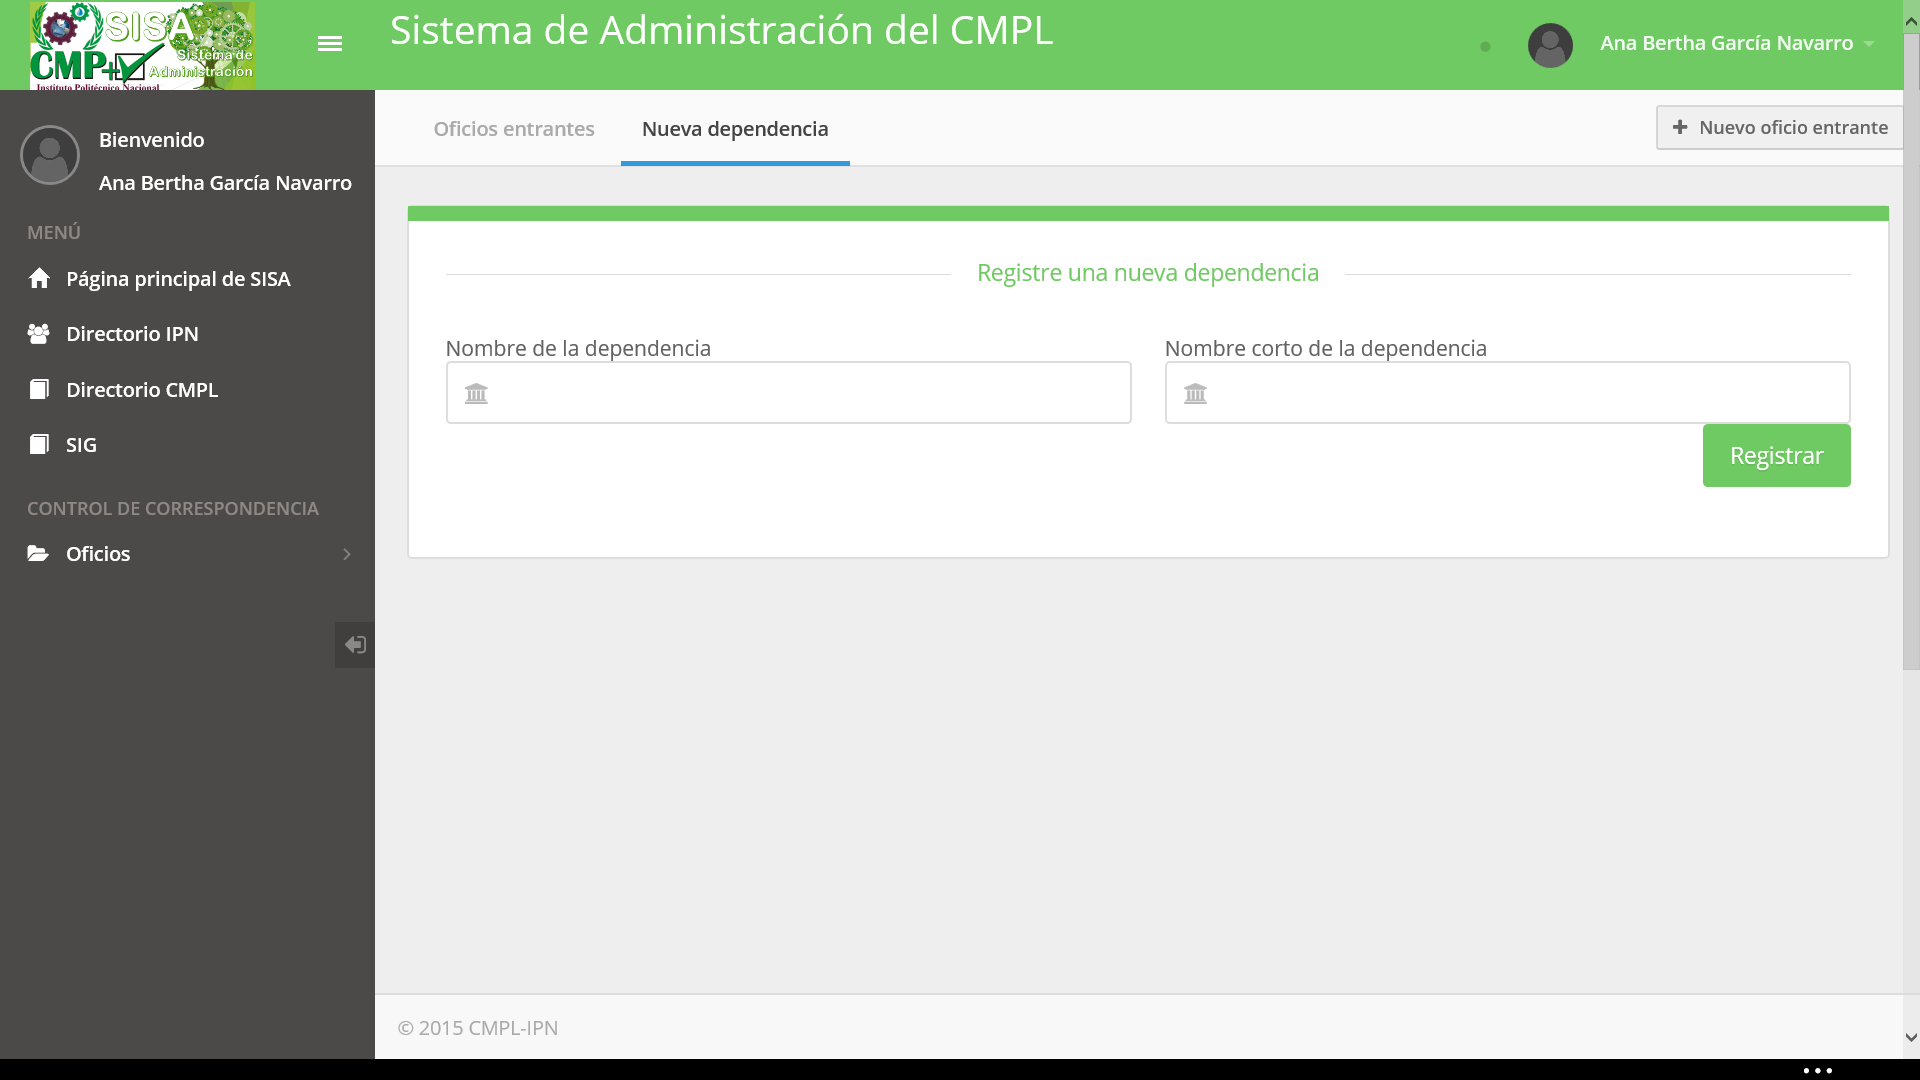
\includegraphics[width=1\textwidth]{Pantallas/NuevaDependencia.png}
		\caption{Pantalla de registro de dependencia que emite de oficios entrantes.}
		\label{fig:NuevaDependencia}
	\end{figure}

\subsubsection{Funcionamiento}
	Esta pantalla funciona de la siguiente manera:
	
	\begin{enumerate}
		\item El usuario ingresa el nombre y el acrónimo de la dependencia que emite.
		\item El usuario da clic en ``Registrar''.
		\item La aplicación valida que todos los campos requeridos estén llenos.
		\item La aplicación registra la información ingresada.
		\item La aplicación vuelve a la pantalla de la figura \ref{fig:Wizard1DatosDelRemitente}, con el registro de la nueva dependencia.
	\end{enumerate}

\subsubsection{Problemas que resuelve}
Esta pantalla ayuda a mitigar las causas que dan origen a los siguientes problemas:

	\begin{itemize}
		\item Es complicado consultar todos los oficios que una dependencia ha enviado al CMPL.
	\end{itemize}

\subsubsection{Pantallas relacionadas}
Está pantalla se relaciona con las siguientes figuras de pantallas:
	\begin{itemize}
		\item \ref{fig:Wizard1DatosDelRemitente}
	\end{itemize}